\subsection{Descrição aproximada das oscilações betatron}\label{sec:2.8}
Para diversos propósitos, é conveniente -- e suficiente -- aproximar o movimento betatron por uma oscilação harmônica simples. Considera-se a oscilação
\begin{align}
	x = A\ cos(s/ \lambdabar - \vartheta)\label{eq:2.66}
\end{align}
onde $\lambdabar$ é constante (o comprimento de onda reduzido). Uma oscilação completa é realizada quando $s$ avança por um comprimento de onda $2\pi \lambdabar$. É claramente conveniente pensar na oscilação pseudo-harmônica da equação \eqref{eq:2.43} como apenas uma onda senoidal com um comprimento de onda localmente variável -- se a variação de amplitude for ignorada. E, com tanto que $\beta$ não varie tão abruptamente, pode-se esperar que esta é uma aproximação razoável para o movimento real se a equação \eqref{eq:2.66} for utilizada com um $\lambdabar$ escolhido apropriadamente. Supõe-se que o número $\beta_n$ seja definido de forma a ser uma constante que dará o mesmo avanço de fase em uma revolução que a real função $\beta$. Isto é, $\beta_n$ é definido por
\begin{align}
	\int\limits_{0}^{L} \frac{ds}{\beta} = \frac{L}{\beta_n}\label{eq:2.67}
\end{align}
e é chamado de valor típico de $\beta$. Então, a oscilação
\begin{align}
	x = A\ cos(s/\beta_n + \vartheta)\label{eq:2.68}
\end{align}
irá -- com $A=a\sqrt{\beta_n}$ -- estar de acordo com a trajetória real pelo menos uma vez a cada revolução; e, em particular, irá estar, na média, em fase com a oscilação real. Na \autoref{fig:fig15} estão representadas uma das trajetórias da \autoref{fig:fig12} junto com sua aproximação obetida pela equação \eqref{eq:2.66}.

\begin{figure}[!htb]
	\centering
	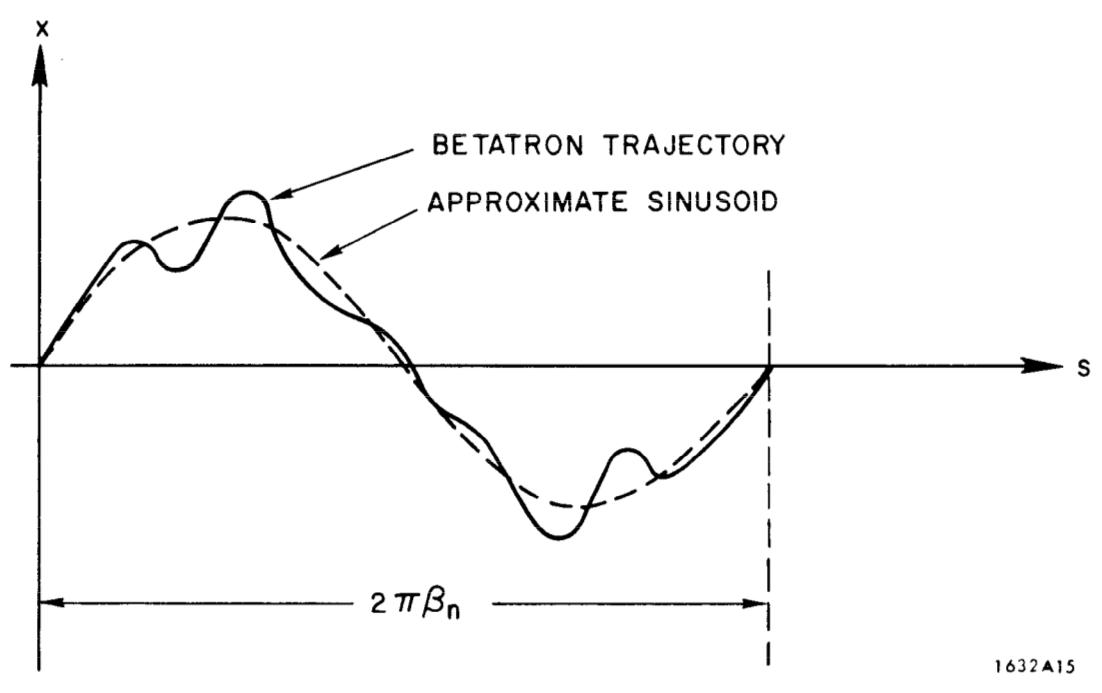
\includegraphics[width=0.7\linewidth]{./Figuras/fig15.jpeg}
	\caption{Aproximação da trajetória betatron.  ------ trajetória betatron; -- -- --  aproximação senoidal. Retirado de \cite{sands1970physics}.}
	\label{fig:fig15}
\end{figure}

É conveniente lembrar que, pela equação \eqref{eq:2.67}, $\frac{1}{\beta_n}$ é apenas a média de $\frac{1}{\beta}$ ao redor do anel:
\begin{align}
	\frac{1}{\beta_n} = \left \langle \frac{1}{\beta} \right \rangle
\end{align}

Pela definição de $\nu$ (equação \eqref{eq:2.60}), tem-se
\begin{align}
	\frac{L}{\beta_n} = 2\pi \nu
\end{align}

O raio efetivo de curvatura da órbita é dado por
\begin{align}
	R = \frac{L}{2\pi}
\end{align}
então pode-se também definir como
\begin{align}
	\beta_n = \frac{R}{\nu}\label{eq:2.72}
\end{align}

Note que $\beta_n$ não é igual à média de $\beta$, apesar de que também não é muito diferente se as ondulações de $\beta$ não forem muito grandes. Vale ressaltar que $\beta_n$ é tal que a sintonia da máquina é mantida.

\begin{proof}
	Pela definição de $\nu$ e $\beta_n$ dadas respectivamente pelas equações \eqref{eq:2.60} e \eqref{eq:2.67},
	\begin{align*}
		\nu &= \frac{1}{2\pi} \int\limits_{0}^{L}\frac{ds}{\beta}\\
			&= \frac{1}{2\pi} \frac{L}{\beta_n}\\
		\therefore \frac{L}{\beta_n} &= 2\pi \nu
	\end{align*}
	
	Mas $R = L/2\pi$. Então,
	\begin{align*}
		\frac{L}{\beta_n} &= 2\pi \nu\\
		\therefore \beta_n &= \frac{L}{2\pi \nu}\\
						   &= \frac{R}{\nu}
	\end{align*}
\end{proof}

A variação de tempo da trajetória aproximada da equação \eqref{eq:2.68} é descrita como
\begin{align}
	x = A\ cos(\nu \omega_r t - \vartheta)
\end{align}
com $\omega_r = c/R$.

\begin{proof}
	Pela equação \eqref{eq:2.68}, $x = A\ cos(s/\beta_n - \vartheta)$. Agora, considerando como 0 a coordenada $s$ de referência, pela equação \eqref{eq:2.48}:
	\begin{align*}
		x &= A\ cos(s/\beta_n - \vartheta)\\
		  &= A\ cos(ct/\beta_n - \vartheta)\\
		  &= A\ cos(\nu c t/R - \vartheta)
	\end{align*}
	
	Definindo $\omega_r = c/R$, tem-se
	\begin{align*}
		x &= A\ cos(\nu \omega_r t - \vartheta)
	\end{align*}
	c.q.d.
\end{proof}

A frequência angular $\nu \omega_r$ é chamada de frequência betatron e será denominada por $\omega_\beta$. Note que, quando a trajetória aproximada é observada em um ponto fixo do anel, sua variação de tempo é indistinguível da trajetória real -- basta comparar com a equação \eqref{eq:2.64}.

A aproximação realizada nesta Seção não é adequada para vários cálculos dos efeitos do anel, mas de fato providencia a única abordagem rastreável para a análise de alguns dos efeitos coletivos que envolvem um número grande de elétrons armazenados.